\documentclass[a4paper, top=10mm]{article}
\usepackage[french]{babel}
%for writing from the top
\usepackage{fullpage}
%for math
\usepackage{amsmath}
\usepackage{mathrsfs}
\usepackage{amsthm}
%for images
\usepackage{graphicx}
%for color
\usepackage{xcolor}
%for title
\title{\textbf{\huge{Le père de famille}}}
\author{Enigme n\textsuperscript{o}1}
\date{20 Janvier 2024}

\newtheorem*{hint}{Hint}

\addtolength{\voffset}{-2cm}
\addtolength{\textheight}{5cm}


\begin{document}
	\maketitle
	
	\huge
	Le père de Tom à trois fils:
	\begin{enumerate}
		\item Tic
		\item Tac
		\item ?
	\end{enumerate}

	\vspace{3cm}
	
	\begin{center}
		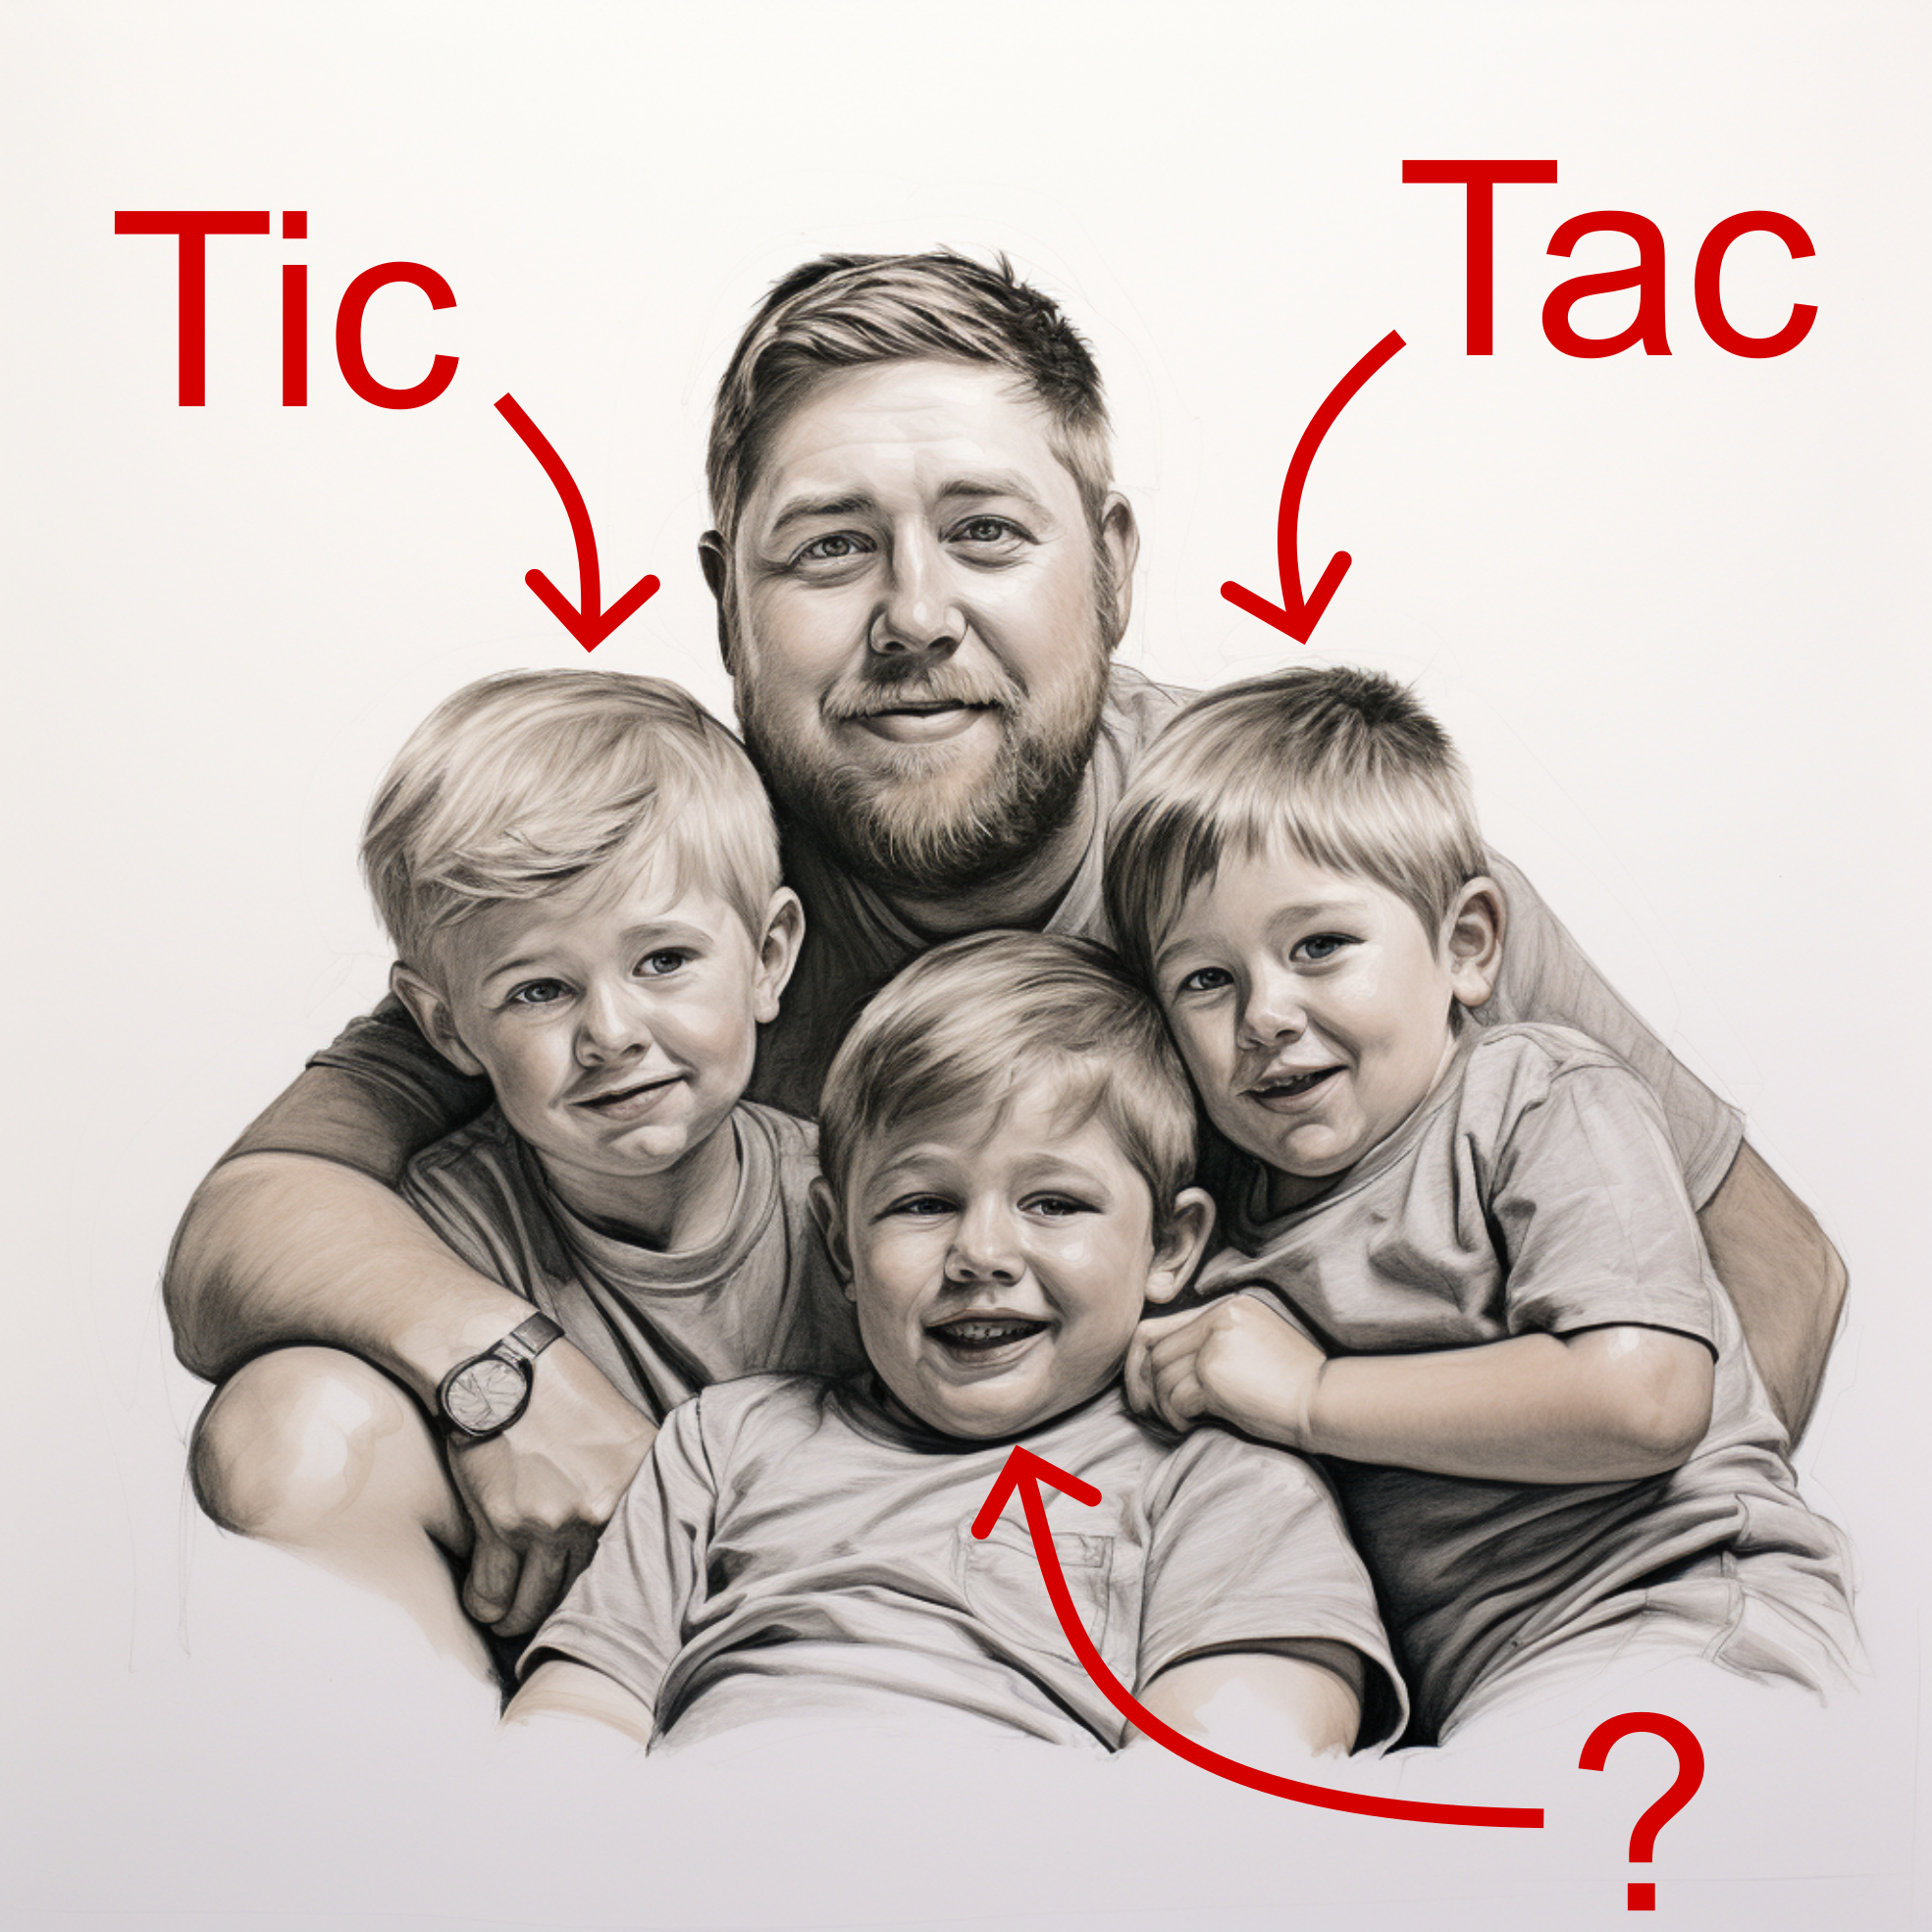
\includegraphics[height=400pt]{01family_labeled.png}
	\end{center}
	
\end{document}